\documentclass[11pt]{article}
\usepackage[T1]{fontenc}
\usepackage{lmodern}
\usepackage[margin=1in]{geometry}
\usepackage{amsmath,amssymb,amsthm,booktabs,array,graphicx,microtype}
\usepackage[obeyspaces,spaces]{url}
\usepackage[hidelinks]{hyperref}
\hypersetup{pdftitle={When does a negative assay exclude a finite target count?},
 pdfsubject={Sharp false-exclusion bounds for native-reference reporting rules}}
\usepackage[numbers,sort&compress]{natbib}
\usepackage{caption}
\makeatletter
\let\tableinput\@@input
\makeatother
\DeclareUrlCommand\lean{\urlstyle{tt}}
\captionsetup{font=small,labelfont=bf}
\setlength{\parskip}{3pt}
\setlength{\emergencystretch}{2em}
\newtheorem{theorem}{Theorem}[section]
\newtheorem{proposition}[theorem]{Proposition}
\newtheorem{corollary}[theorem]{Corollary}
\newtheorem{lemma}[theorem]{Lemma}
\theoremstyle{remark}\newtheorem{remark}[theorem]{Remark}
\newcommand{\E}{\mathbb E}
\newcommand{\Prob}{\mathbb P}
\newcommand{\Neg}{\mathcal N}

\title{When does a negative assay exclude a finite target count?\\[4pt]
\large Sharp false-exclusion bounds for native-reference reporting rules}
\author{}
\date{17 September 2026}

\begin{document}
\maketitle
\vspace{-1.8em}
\begin{abstract}
A negative readout need not exclude targets in the original specimen when
extraction failures are shared across targets and splitting consumes material.
We study a finite, well-mixed specimen with conditionally independent target
paths and arbitrary dependence between two preparation recoveries. A sharp
moment bound reduces the all-negative probability to four recovery states. An
explicit reporting rule accepts each of $m$ independent native-reference pairs
whenever at least one reference is recovered, and issues a count-exclusion
certificate only if the future assay is also negative. For balanced effective
fractions $a$, the exact worst-case probability of a false certificate is
$G_m((1-a)^K)$, where $G_m(H)=\max_{0\le z\le1}z^m[1-(1-H)z]$ has a closed
two-branch formula; no equality of marginal recovery means is needed, and an
explicit source attains the value. We then quantify four things that a reporting
rule must survive. Reusing one calibration across $T$ independent specimens has
an exact familywise value with an irreducible floor $1-(1-H)^T$, so a five
percent familywise level is \emph{unreachable} for two specimens in the worked
design however many references are bought. Replacing the exactly-one reference
input by Poisson loading of mean $\lambda$ leaves the guarantee intact for
$\lambda\le1$, has a closed sharp value $d_\lambda^{\,m}G_m((1-2a)^K)$ under an
explicit rational criterion, and in general reduces to a one-dimensional
concave-envelope problem; heavy loading destroys the guarantee outright. An event-specific
allowance for observation-law mismatch replaces a product-coupling bound that
was an order of magnitude looser. Spurious control positives admit an exact
reduction to the same scalar problem, and the resulting specificity budget --- a
pair false-positive rate below about $1/300$ --- is the binding practical
constraint. Finally, imposing equal means and nonnegative covariance moves the
feasibility threshold from $(1-a)^K$ to $(1-2a)^K$, which makes an otherwise
impossible exclusion attainable. The central chain and the new batch, false
positive and Poisson results are mechanized in Lean~4; biological transport
remains an experimental premise.
\end{abstract}

\section{Question and contribution}\label{sec:intro}
Given limited specimen volume, uncertain extraction and recovery, and shared
interference, when does a negative result justify exclusion---and should the next
experiment use more specimen, another extraction, another well, or a different
measurement?

The relevant denominator is the original sampled specimen. Increasing the number
of wells does not itself increase the amount of original material observed, and
recoveries in separate preparations need not be independent. We ask a bounded
version of this decision problem: how should a fixed specimen be allocated to one
or two preparations, and what explicit native-reference reporting rule permits a
uniform exclusion guarantee? The target is the count $N$ in that specimen.
Excluding $N\ge K$ means reporting $N<K$; it does not establish sterility,
patient absence, source concentration, or a population prevalence.

Multistage detection errors and their identifiability are established subjects.
Guillera-Arroita et al.\ \cite{guillera2017} analyze detection errors at multiple
levels and the additional observations needed to distinguish model parameters.
Smart et al.\ \cite{smart2016} and Lugg et al.\ \cite{lugg2018} develop
cost-aware environmental-DNA sampling designs. Their survey objectives differ
from the finite-specimen, worst-case reporting probability studied here. Bounds
on the expectation of a convex function through its values at the vertices of a
box are classical \cite{madansky1959,hoeffding1955}, as is the fact that an
extremal law for finitely many moment constraints needs few support points
\cite{karlin1966,winkler1988}; our corner and envelope arguments are applications,
not new convex-order principles. Binary performance-demonstration tests also
explicitly trade sample size against acceptance risk \cite{leber2019}, and
multiplicity control for families of decisions has a standard vocabulary
\cite{benjamini1995}.

Our contribution is the complete connection from conserved target paths to a
sharp allocation bound and an observable native-reference rule, followed by an
exact accounting of what happens when the four premises a laboratory is most
likely to break are relaxed one at a time. Concretely:

\begin{enumerate}\itemsep2pt
\item A sharp four-state envelope for the all-negative probability
  (Theorem~\ref{thm:envelope}) and the exact worst-case error of the
  at-least-one native-reference gate, $G_m((1-a)^K)$, with an attaining source
  (Theorems~\ref{thm:scalar} and~\ref{thm:main}).
\item The exact familywise value when one calibration is reused for $T$
  independent specimens, its irreducible floor, and the resulting impossibility
  and reachability statements (Section~\ref{sec:batch}).
\item Poisson-loaded native references: an exact reduction to a one-dimensional
  concave-envelope problem for every loading mean, a closed form under a sharp
  and checkable criterion, a proof that loading means at most one cannot break
  the original guarantee, and a counterexample showing that heavy loading does
  (Section~\ref{sec:poisson}).
\item An event-specific allowance for observation-law mismatch that is
  evaluated exactly on a five-point critical set, and an exact reduction of the
  spurious-positive problem to the same scalar maximum, which converts a vague
  specificity concern into a number (Section~\ref{sec:robust}).
\item A sharp value under equal means and nonnegative covariance, whose floor is
  $(1-2a)^K$ rather than $(1-a)^K$; the restriction converts an impossible
  exclusion into a merely expensive one (Section~\ref{sec:constrained}).
\end{enumerate}

The mathematical scope throughout is a prescribed family of reporting policies,
not unrestricted optimal experimental design. We provide ordinary proofs, with a
machine-checked core; Appendix~\ref{app:formal} states exactly which claims are
mechanized. The analysis is conditional on a stated experimental model. No
clinical validation is claimed and no priority claim about a named open
conjecture is made.

\section{Material, recovery and the reporting event}\label{sec:model}
\subsection{A finite specimen and shared preparation states}
Let $N$ targets be uniformly located in a homogeneous specimen of volume $V_0$.
Two disjoint effective fractions $a,b\ge0$ satisfy $a+b\le1$. They combine usable
original volume and downstream coverage. With available volume $V\le V_0$,
representative setup loss $\ell$ per preparation and full downstream coverage,
balanced splitting gives
\begin{equation}\label{eq:volumes}
a=b=\frac{V/2-\ell}{V_0},\qquad
s=\frac{V-\ell}{V_0}
\end{equation}
for the split and single-preparation designs, respectively. Each formula is used
only when its usable volume is nonnegative. Representative loss means that the
discarded volume carries targets with the same allocation law as the retained
volume. Selective retention or changed inhibitor concentration is not
automatically represented by subtracting $\ell$.

A recovery state $(X,Y)\in[0,1]^2$ is drawn once for the specimen. Conditional on
that complete state, the targets have independent allocation and retention marks.
Recovery is shared by all targets allocated to a preparation; $X$ and $Y$ may be
dependent. The same recovery law must apply at the compared volumes and at every
admitted target count. Abundance-dependent recovery, aggregation and competition
are outside this contract unless incorporated in a new source model.

For one target, the five terminal path masses are
\begin{equation}\label{eq:paths}
1-a-b,\quad a(1-X),\quad aX,\quad b(1-Y),\quad bY.
\end{equation}
They represent unprocessed material, loss and detection in the first preparation,
and loss and detection in the second. They are nonnegative and sum to one.
Summing histories with no detection gives
\begin{equation}\label{eq:source}
R_N(a,b)=\E[(1-aX-bY)^N].
\end{equation}
The expectation is taken \emph{after} the $N$-target product. Taking a product of
marginal expectations would incorrectly renew the preparation state for each
target. For $N=0$ the probability is one. Because the base lies in $[0,1]$,
$R_N\le R_K$ whenever $N\ge K$.

For specificity, the formal model uses any finite mixture of real-valued recovery
states. The analytic arguments also hold for any probability law on the unit
square by integrating the same pointwise inequalities. The latter
measure-theoretic extension is not part of the mechanized claim.

\subsection{Native references and independence}\label{sec:refs}
Each reference pair contains one known native target in each usable preparation
input, before the native recovery gate. Conditional on its state $(X,Y)$, the two
reference counts $A,B\in\{0,1\}$ are independent Bernoulli outcomes. Thus
\begin{equation}\label{eq:reference}
\Prob((A,B)=00,10,01,11\mid X,Y)
=((1-X)(1-Y),X(1-Y),(1-X)Y,XY).
\end{equation}
Pairs are independent draws from the same state population, and the future target
specimen is another independent draw. This assumption concerns independent
experiments, not unconditional independence within a pair. A common unmodeled
batch effect across reference pairs and the specimen can invalidate it.
Section~\ref{sec:poisson} replaces the exactly-one input count by an explicit
stochastic loading model, and Section~\ref{sec:robust} prices the failure of the
observation law itself.

The references must transport to native targets at the selected volumes, matrices
and target forms. Known input counts, accurate terminal counting and absence of
competition are required. A soluble spike added downstream does not supply this
contract. Setup-volume loss is counted in $a,b,s$, rather than counted a second
time in reference recovery. External reference material is separate from the
limited target specimen.

\subsection{A prespecified complete-event guarantee}
Fix $K\ge1$, $m\ge1$, an action and error budget $\alpha$ before the experiment.
Let $\mathcal A_m$ be the event that every reference pair has at least one
recovery, and let $\Neg$ be the event that the future target assay is all
negative. The rule certifies $N<K$ only if $\mathcal A_m$ occurs, $\Neg$ occurs,
and the action's proved bound is at most $\alpha$. Otherwise it issues no such
certificate. Failed or missing references are unresolved; invalid records are not
converted to passes. The guarantee is
\begin{equation}\label{eq:error}
\sup_{\mathcal L(X,Y),\,N\ge K}\Prob(\mathcal A_m\cap\Neg)\le\alpha.
\end{equation}
This is one complete experiment, including its reference campaign and one future
specimen. Blank-certificate probability is reported separately as usefulness.

\section{A sharp four-state reduction}\label{sec:corners}
Write $p_1=\E X$, $p_2=\E Y$, $q=\E[XY]$. Feasibility implies
\begin{equation}\label{eq:feasible}
\max(0,p_1+p_2-1)\le q\le\min(p_1,p_2),
\end{equation}
since $XY\ge0$, $XY\le X,Y$, and $(1-X)(1-Y)\ge0$.

\begin{theorem}[Sharp moment envelope]\label{thm:envelope}
For $N\ge K\ge1$ and $a,b\ge0$ with $a+b\le1$,
\begin{align}\label{eq:envelope}
R_N(a,b)\le B_K(a,b):={}&1-p_1-p_2+q\notag\\
&+(p_1-q)(1-a)^K+(p_2-q)(1-b)^K+q(1-a-b)^K.
\end{align}
At $N=K$ equality is attained by the masses
\begin{equation}\label{eq:cornerlaw}
(c_{00},c_{10},c_{01},c_{11})=(1-p_1-p_2+q,\,p_1-q,\,p_2-q,\,q)
\end{equation}
on $(0,0),(1,0),(0,1),(1,1)$. The same law attains the envelope for every
allocation.
\end{theorem}
\begin{proof}
On the unit square, $(1-ax-by)^K$ is convex in each coordinate: for $K=1$ it is
affine, and for $K\ge2$ its coordinate second derivatives are nonnegative.
Successive endpoint interpolation in $x$ and then $y$ bounds it above by
\[
(1-x)(1-y)+x(1-y)(1-a)^K+(1-x)y(1-b)^K+xy(1-a-b)^K.
\]
Taking expectations gives \eqref{eq:envelope}, and count monotonicity covers
$N\ge K$. The masses in \eqref{eq:cornerlaw} are nonnegative by
\eqref{eq:feasible}, sum to one, and have moments $p_1,p_2,q$. At every corner
the interpolation is exact.
\end{proof}

The integrated reference law \eqref{eq:reference} has precisely the four masses
\eqref{eq:cornerlaw}, even when native recovery is continuously valued. Thus
paired reference outcomes measure the moments relevant to the bound without
asserting that actual recoveries are binary. This is the reason the calibration
experiment and the bound speak the same language.

\section{The at-least-one gate and its exact error}\label{sec:gate}
Define
\[
w=p_1+p_2-q=\Prob(A\lor B),\qquad q=\Prob(A=B=1).
\]
Then $0\le w\le1$, and independent reference pairs give
$\Prob(\mathcal A_m)=w^m$. Independence from the future specimen yields the
complete-event identity
\begin{equation}\label{eq:joint}
\Prob(\mathcal A_m\cap\Neg)=w^m R_N(a,b).
\end{equation}

For balanced $a=b\le1/2$, set
\begin{equation}\label{eq:HJ}
H=(1-a)^K,\qquad J=(1-2a)^K .
\end{equation}
The envelope simplifies to
\begin{equation}\label{eq:reduction}
B_K(a,a)=1-w(1-H)-q(H-J)\le1-w(1-H),
\end{equation}
because $0\le J\le H\le1$. No equality of $p_1,p_2$ is used. Both $H$ and $J$
recur throughout: $H$ is the miss probability of a source in which exactly one
preparation recovers, and $J$ that of a source in which both do.

\begin{theorem}[Scalar maximum]\label{thm:scalar}
For an integer $m\ge1$ and $0\le H\le1$,
\begin{equation}\label{eq:G}
G_m(H):=\max_{0\le z\le1}z^m[1-(1-H)z]
=\begin{cases}
H,& H\ge1/(m+1),\\[2pt]
\displaystyle\frac{m^m}{(m+1)^{m+1}(1-H)^m},&H<1/(m+1).
\end{cases}
\end{equation}
The maximizer is $z_*=1$ in the first branch and $z_*=m/[(m+1)(1-H)]$ in the
second. $G_m$ is nondecreasing in $H$ and nonincreasing in $m$.
\end{theorem}
\begin{proof}
At $H=1$ the function is $z^m$, with maximum one. For $H<1$ its derivative is
$z^{m-1}\{m-(m+1)(1-H)z\}$. If $H\ge1/(m+1)$ this is nonnegative throughout
$[0,1]$. Otherwise its sign changes from nonnegative to nonpositive at $z_*$,
which lies strictly between zero and one. Evaluating at the respective
maximizers gives \eqref{eq:G}, and the branch values agree at equality.
Monotonicity in $H$ holds because $G_m$ is a maximum of functions affine and
nondecreasing in $H$; monotonicity in $m$ holds because $z^m$ is nonincreasing in
$m$ on $[0,1]$.
\end{proof}

\begin{theorem}[Sharp calibrated count exclusion]\label{thm:main}
Under the model of Section~\ref{sec:model}, balanced fractions $0\le a\le1/2$ and
integers $K,m\ge1$ satisfy
\begin{equation}\label{eq:main}
\sup_{\mathcal L(X,Y),\,N\ge K}\Prob(\mathcal A_m\cap\Neg)=G_m\big((1-a)^K\big).
\end{equation}
The supremum is attained in the finite-mixture class, without any constraint on
the marginal means. At a fixed source, blank-certificate probability is $w^m$
when the design is eligible to certify.
\end{theorem}
\begin{proof}
Equations \eqref{eq:joint}--\eqref{eq:reduction} and Theorem~\ref{thm:scalar}
give the upper bound. For attainment choose $N=K$ and corner masses
\begin{equation}\label{eq:attainer}
(1-z_*,\ z_*/2,\ z_*/2,\ 0),
\end{equation}
an admissible law with $w=z_*$, $q=0$ and equal means $z_*/2$. Its source miss
probability is $1-z_*+z_*H$ and its gate probability is $z_*^m$; their product is
$G_m(H)$. At $N=0$ all target records are negative, so \eqref{eq:joint} reduces
to $w^m$.
\end{proof}

\begin{corollary}[Three pairs and two targets]\label{cor:cubic}
For $K=2$, $m=3$ and balanced $a\le1/2$, the sharp complete-event error is
$(1-a)^2$. An attaining law assigns probability $1/2$ to each single-good corner.
\end{corollary}
\begin{proof}
$H=(1-a)^2\ge1/4$, so the endpoint branch applies. Equivalently the bound follows
from the nonnegative identity
\[
H-z^3[1-z(1-H)]=\frac{(1-z)^2(3z^2+2z+1)}4+\big(H-\tfrac14\big)(1-z^4).\qedhere
\]
\end{proof}

\begin{figure}[!htb]
\centering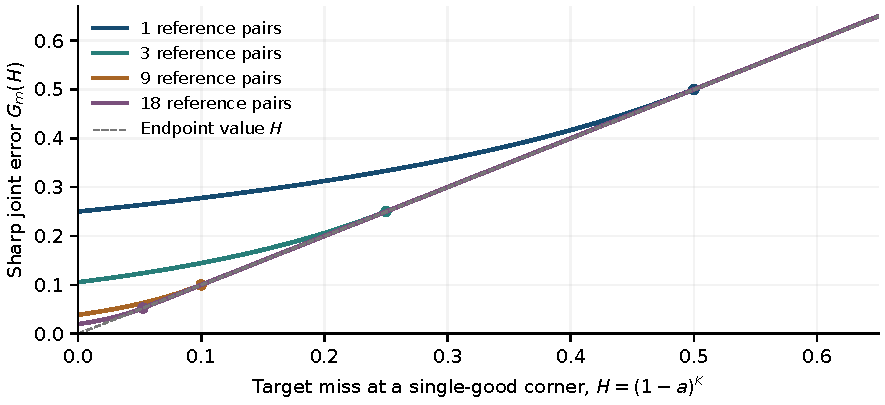
\includegraphics[width=.92\linewidth]{figures/gate_bound.pdf}
\caption{Exact worst-case error for the prespecified gate family. Dots mark
$H=1/(m+1)$, separating an interior adverse source from a source that passes
calibration surely. The dashed line is the irreducible endpoint value.}
\label{fig:bound}
\end{figure}

\subsection{Why the larger gate is useful}
Requiring \emph{exactly} one recovered reference per pair would give acceptance
$r^m$, where $r=p_1+p_2-2q=w-q$. That event is a subset of $\mathcal A_m$. For
balanced allocation its envelope is $1-r(1-H)-q(1-J)\le1-r(1-H)$, and the same
$q=0$ source \eqref{eq:attainer} attains $G_m(H)$. Consequently the larger gate
increases blank-report availability while preserving the entire sharp worst-case
curve. It does not decrease actual error pointwise: accepting more records may
increase the actual probability of issuing a false certificate at a given source.

At independent Bernoulli recovery $p_1=p_2=0.8$, $q=0.64$, three pairs give
$r^3=0.032768$ against $w^3=0.884736$. Double-positive reference pairs are
favorable observations; rejecting them imposes an unnecessary availability cost.

\begin{figure}[!htb]
\centering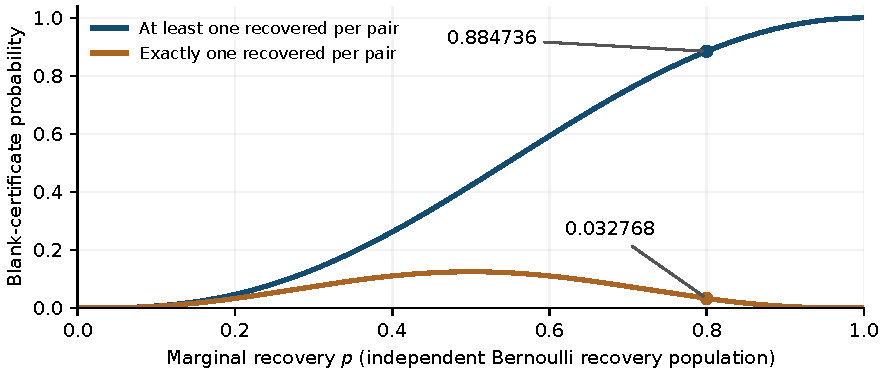
\includegraphics[width=.92\linewidth]{figures/gate_utility.pdf}
\caption{Blank-certificate availability with three pairs in a synthetic
independent Bernoulli recovery population. The gate change uses the same six
external native inputs. Equality of worst-case error does not imply equality of
source-specific error.}
\label{fig:utility}
\end{figure}

\section{Allocation and calibration-policy choices}\label{sec:choice}
\subsection{Balancing is minimax at fixed total coverage}
For unequal fractions define $H_a=(1-a)^K$, $H_b=(1-b)^K$ and
$H_{\max}=\max(H_a,H_b)$. Because $c_{00}=1-w$ and
$c_{10}+c_{01}+c_{11}=w$, the corner envelope is
\[
c_{00}+c_{10}H_a+c_{01}H_b+c_{11}(1-a-b)^K\le 1-w+wH_{\max},
\]
using $(1-a-b)^K\le\min(H_a,H_b)$. The sharp complete-event error is therefore
$G_m(H_{\max})$: to attain it, put mass $1-z_*$ at $(0,0)$ and mass $z_*$ at the
single-good corner belonging to the \emph{smaller} allocated fraction, which is
permitted when marginal means are unrestricted. Since $G_m$ is nondecreasing in
$H$ and balancing maximizes the smaller fraction at fixed $a+b$, balancing
minimizes the sharp error.

If equal marginal means are imposed then $c_{10}=c_{01}$ and the sharp expression
instead uses $H_{\mathrm{avg}}=(H_a+H_b)/2$, attained by the symmetric law
\eqref{eq:attainer}. Convexity of $t\mapsto(1-t)^K$ again favors balance. These
are different source classes; the unrestricted result must not be justified by
silently imposing equal means.

\subsection{A fair single-preparation comparator}
For a single preparation with effective fraction $s$, put $u=(1-s)^K$ and
$p=\E X$. The one-coordinate chord inequality gives $R_N(s)\le1-p(1-u)$. Require
all $m$ independent native reference preparations for that protocol to recover.
Its complete error and blank utility satisfy
\begin{equation}\label{eq:single}
\sup_{\mathcal L(X),\,N\ge K}\Prob(\text{references pass}\cap\Neg)=G_m(u),
\qquad \Prob_0(\text{certificate})=p^m.
\end{equation}
The upper bound is Theorem~\ref{thm:scalar}; a Bernoulli recovery population with
success probability $z_*$ attains it. No second protocol or equal-mean premise is
needed. Here $m$ references mean $m$ independent latent draws: six readouts
nested within three shared-state pairs are not six independent references.

\begin{table}[tb]
\centering\small
\caption{Finite policy menu at $K=2$, $a=.45$, $s=.95$. Errors are uniform sharp
bounds; utilities use the synthetic independent $.8$ recovery population only.
Reference costs count native inputs and preparations.}
\label{tab:menu}
\begin{tabular}{@{}lrrrr@{}}\toprule
Policy & Joint error & Blank utility & Refs. & Specimen preps.\\\midrule
\tableinput policy_rows.tex
\bottomrule\end{tabular}
\end{table}

The discordance choice in Table~\ref{tab:menu} is removed from the efficient
menu: the at-least-one rule has the same uniform error and cost and greater
utility at the displayed operating point. The remaining three choices trade
error, availability and cost, and none dominates the others in those objectives.
With a six-reference ceiling and a blank-availability requirement $\beta=.8$ on
the subclass of independent protocol recoveries each of mean at least $.8$, only
the pair rule in this menu qualifies. A stricter error target can instead favor a
single-preparation success gate, at reduced availability. Positive blank utility
is impossible uniformly over the unrestricted recovery class, which includes
total failure.

\subsection{Known moments answer a separate question}
When equal means $p$ and cross-moment $q$ are known, the single and balanced
two-preparation bounds are
\[
B_1=1-p+p(1-s)^K,\qquad
B_2=1-2p+q+2(p-q)(1-a)^K+q(1-2a)^K,
\]
whose difference is $pA-qC$ with $A=1+(1-s)^K-2(1-a)^K$ and
$C=1-2(1-a)^K+(1-2a)^K$. At $K=2$, $p=.8$, $s=.95$, $a=.45$, splitting wins
exactly when $q<106/135\approx.785185$. For $q=.64$ its risk is $.1432$ against
$.202$; for $q=.79$ it is $.20395$ and the single preparation wins. These
known-moment risks exclude calibration uncertainty and must not be interchanged
with Table~\ref{tab:menu}.

\subsection{What additional resources change}
Under \eqref{eq:source}, another well with unchanged unique effective coverage
and shared recovery leaves the risk unchanged. Assaying unused extract or
changing inhibition changes a premise and can help. Another extraction changes
coverage, setup loss and joint recovery. More original specimen changes feasible
fractions only under an applicable sampling and volume-transport contract. A
different measurement requires a new validated observation or recovery law.
These results do not choose actions after an arbitrary history of previous target
negatives; such conditioning requires a separate sequential analysis.

\section{Calibration cost and a worked exclusion}\label{sec:examples}
For $H>0$, the endpoint $G_m(H)=H$ is reached exactly when $m\ge1/H-1$, so the
smallest permitted pair count is $\max\{1,\lceil1/H\rceil-1\}$. At full balanced
coverage $a=1/2$ this requires $m\ge2^K-1$. That exponential cost is the cost of
reaching the \emph{exact endpoint}, not of meeting every fixed error tolerance.

For fixed $m$ and fixed $a>0$, increasing $K$ sends $H$ to zero and leaves the
floor
\[
c_m=\frac{m^m}{(m+1)^{m+1}},\qquad (m+1)c_m\longrightarrow e^{-1}.
\]
In the interior branch $G_m(H)=c_m(1-H)^{-m}$, which for fixed $m$ equals
$c_m[1+mH+O(H^2)]$; no uniform expansion in growing $m$ is asserted. At $K=2$ we
have $H\ge1/4$, so this balanced gate family cannot provide a universal
five-percent certificate regardless of the number of reference pairs.
Section~\ref{sec:constrained} shows that this particular impossibility is a
property of the unrestricted source class and not of the design.

\subsection{A five-percent example with a higher target threshold}
Consider a synthetic $V_0=V=1\,\mathrm{mL}$ specimen, representative loss
$\ell=.05\,\mathrm{mL}$ per preparation and full downstream coverage. Two inputs
of $.5\,\mathrm{mL}$ leave $.45\,\mathrm{mL}$ usable each, so $a=.45$. The target
unit is one native analyte unit obeying the independent-marking model, not an
organism or clinical case by implication. Table~\ref{tab:thresholds} uses exact
rational values behind the rounded displays.

\begin{table}[tb]
\centering\small
\caption{Balanced $a=.45$ at error budget $.05$. Utility assumes independent
Bernoulli $.8$ recoveries, hence $w=.96$. Each accepted reference pair needs at
least one recovery. ``Infeasible'' refers to this policy family and this source
class.}
\label{tab:thresholds}
\begin{tabular}{@{}rrrrrr@{}}\toprule
Null $N\ge K$ & $H=.55^K$ & Min. pairs & Joint bound & Blank utility & Refs.\\\midrule
\tableinput threshold_rows.tex
\bottomrule\end{tabular}
\end{table}

For $K=6$, nine pairs suffice and eight do not: the reporting bound is
$G_9((11/20)^6)\approx.04987721425$, and minimality follows because
$z^m[1-(1-H)z]$, hence its maximum, is nonincreasing in $m$ on $0\le z\le1$.
Passing the reference gate and obtaining an all-negative specimen result permits
the report ``fewer than six target units in the original specimen.'' It does not
establish zero targets. The cost is 18 external native inputs, 18 reference
preparations and readouts, nine independent paired latent draws, and two specimen
preparations and readouts. Reference-input volumes must match the preparation
protocol; in the illustrated split architecture this is $18\times.5\,\mathrm{mL}$
of external matched input matrix, distinct from the $1\,\mathrm{mL}$ target
specimen.

The blank-certificate probability at the synthetic operating point is
$.96^9\approx.692534$. For nonblank $N<6$, the specified Bernoulli population
gives
\begin{equation}\label{eq:nonblank}
\Prob_N(\text{certificate})=.96^9\big[.04+.32(.55)^N+.64(.1)^N\big],
\end{equation}
which falls from $.692534$ at $N=0$ to $.038859$ at $N=5$. This quantity, rather
than blank utility, describes low-count reporting. A failed gate, missing or
invalid record, insufficient resource budget or positive target result gives no
exclusion certificate. The design and threshold are fixed before calibration; the
guarantee does not cover searching many gates and reporting whichever happens to
pass.

The margin of this example below $.05$ is only $.000122786$. The three sections
that follow ask what that margin survives.

\section{Reusing one calibration across a batch}\label{sec:batch}
\subsection{Three questions that must be separated}
A laboratory that has paid for $m$ reference pairs will want to use them for more
than one specimen. Three distinct questions arise, and conflating them is the
main way a correct per-experiment guarantee becomes an incorrect batch claim.

\begin{enumerate}\itemsep2pt
\item \emph{Per-specimen unconditional error.} Reusing a gate does not by itself
  invalidate the marginal bound \eqref{eq:main} for each eligible independent
  future specimen from the stated population.
\item \emph{Expected count of false certificates.} If $T_0$ specimens satisfy
  $N_i\ge K$, then the expected number of false certificates is at most
  $T_0\,G_m(H)$ by linearity, even though the reports share a gate.
\item \emph{Familywise error.} The probability of \emph{at least one} false
  certificate in the batch is a different quantity and is not $G_m(H)$.
\end{enumerate}

So the slogan that calibration cannot be amortized is too absolute. It can be
amortized for a specified marginal claim, with shared-report dependence
acknowledged; it cannot be amortized while silently retaining the original
familywise guarantee.

\subsection{The exact familywise value}
Assume one common gate, the same balanced design for every specimen, and
independent future latent draws and target paths, independent of the references.
Fix the null counts rather than letting batch composition depend on calibration.

\begin{theorem}[Sharp familywise error on reuse]\label{thm:batch}
For $T\ge1$ specimens all satisfying $N_i\ge K$, with $H=(1-a)^K$,
\begin{equation}\label{eq:batchmax}
\sup_{\mathcal L(X,Y),\,N_i\ge K}\Prob\big(\mathcal A_m\cap\{\text{some
specimen reads all negative}\}\big)
=F_{m,T}(H):=\max_{0\le w\le1}w^m\big[1-(1-H)^Tw^T\big].
\end{equation}
For $0\le H<1$, writing $c=(1-H)^T$,
\begin{equation}\label{eq:batchform}
F_{m,T}(H)=
\begin{cases}
1-c,& c\le m/(m+T),\\[2mm]
\dfrac{T}{m+T}\left[\dfrac{m}{(m+T)c}\right]^{m/T},& c>m/(m+T),
\end{cases}
\end{equation}
and $F_{m,T}(1)=1$. At $T=1$ this is $G_m(H)$.
\end{theorem}
\begin{proof}
Condition on the population law. The $T$ specimens are independent, so their
all-negative probabilities $R_i$ satisfy $R_i\le1-(1-H)w$ by
\eqref{eq:reduction} and Theorem~\ref{thm:envelope}; hence
$1-R_i\ge(1-H)w$ and the probability that at least one reads all negative is at
most $1-[(1-H)w]^T$. Multiplying by the independent gate probability $w^m$ gives
the bound \eqref{eq:batchmax}. The corner source \eqref{eq:attainer} with
$z_*$ replaced by $w$ and every $N_i=K$ makes both steps equalities and is
admissible for every $w\in[0,1]$, so the supremum is attained. For the closed
form, the derivative of $w^m(1-cw^T)$ is $w^{m-1}[m-(m+T)cw^T]$, whose unique
positive zero is $w_*=[m/((m+T)c)]^{1/T}$; the two branches correspond to
$w_*\ge1$ and $w_*<1$, and in the interior case the value is
$w_*^m(1-m/(m+T))$.
\end{proof}

\subsection{An impossibility floor, and what remains reachable}
Taking $w=1$ in \eqref{eq:batchmax} gives a bound that no reference budget can
beat.

\begin{corollary}[Irreducible familywise floor]\label{cor:floor}
For every $m\ge1$, $F_{m,T}(H)\ge1-(1-H)^T$, and $F_{m,T}(H)\downarrow1-(1-H)^T$
as $m\to\infty$. Consequently a familywise level $\alpha$ is reachable within
this architecture if and only if $\alpha\ge1-(1-H)^T$.
\end{corollary}
\begin{proof}
The lower bound is the value of the objective at $w=1$, attained by the corner
source with $z_*=1$: that source passes every reference pair surely and each
specimen then misses with probability exactly $H$. For the limit, note that
$F_{m,T}$ is nonincreasing in $m$ (as $w^m$ is), and for $m\ge T(1-c)/c$ the
first branch of \eqref{eq:batchform} applies and gives exactly $1-c$.
\end{proof}

At $a=.45$, $K=6$ the floor for $T=2$ is $1-(1-(11/20)^6)^2=.054595\ldots>.05$.
\emph{No number of reference pairs gives a five percent familywise guarantee for
two such specimens.} This is stronger and cleaner than observing that nine pairs
happen to fail, and it is the exact statement mechanized as
\lean{batch_floor_exceeds} in Appendix~\ref{app:formal}.

\begin{table}[tb]
\centering\small
\caption{Reusing one nine-pair calibration at $K=6$, $a=.45$. The familywise
column evaluates the closed form \eqref{eq:batchform}; the floor column is exact
rational arithmetic and is what decides reachability.}
\label{tab:batch}
\begin{tabular}{@{}rrrl@{}}\toprule
Specimens $T$ & Sharp familywise error, $m=9$ & Floor $1-(1-H)^T$ & Level $.05$ reachable?\\\midrule
\tableinput batch_rows.tex
\bottomrule\end{tabular}
\end{table}

Corollary~\ref{cor:floor} is also constructive, because the floor is decreasing
in $H$ and $H=(1-a)^K$ falls quickly in $K$. At $a=.45$ the largest batch with a
reachable five percent familywise level is $T=1$ for $K=6$, but $T=6$ for $K=8$
(needing $m=96$ pairs), $T=20$ for $K=10$ ($m=330$) and $T=66$ for $K=12$
($m=1070$). Batch reporting is therefore not forbidden; it is priced, and the
price is set by the exclusion threshold rather than by the calibration budget.
Figure~\ref{fig:batch} shows both regimes.

\begin{figure}[!htb]
\centering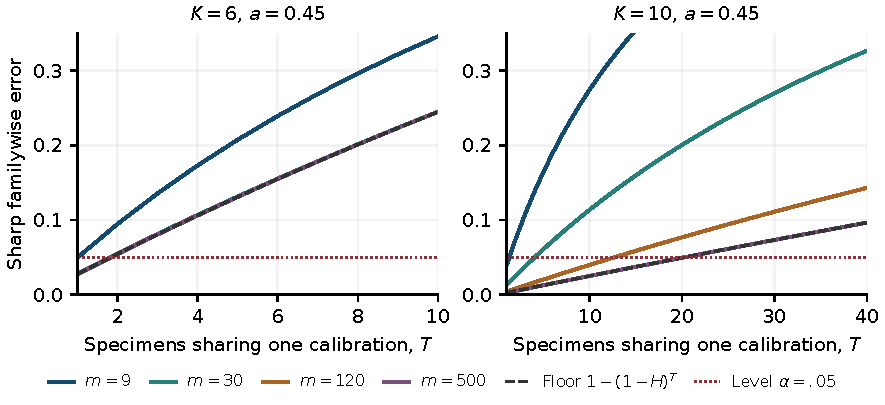
\includegraphics[width=\linewidth]{figures/batch_fwer.pdf}
\caption{Sharp familywise error when one calibration is reused for $T$
independent specimens. Curves are \eqref{eq:batchform}; the dashed line is the
floor of Corollary~\ref{cor:floor}, which no reference budget can cross, and the
dotted line is the level $.05$. At $K=6$ (left) the floor already exceeds the
level at $T=2$; at $K=10$ (right) batches of twenty remain reachable.}
\label{fig:batch}
\end{figure}

\subsection{False discovery rate, and repeated calibration attempts}
Treating a false exclusion as a false discovery does not by itself escape
Corollary~\ref{cor:floor}. Let $D$ be the number of exclusion reports and $V$ the
number of them whose specimens actually satisfy $N_i\ge K$, and put
$\mathrm{FDR}=\E[V/\max(D,1)]$. Then $\mathrm{FDR}\le\Prob(V>0)\le F_{m,T_0}(H)
\le F_{m,T}(H)$, and in an all-null batch $V=D$, so the worst-case FDR over
batch compositions equals the all-null familywise value. A genuinely less
conservative procedure would need per-specimen valid tests or explicitly
conditioned calibration \cite{benjamini1995}; it cannot be inferred from the
present all-pairs gate.

A rare gate must also not be rerun until it passes while the one-campaign error
claim is retained. With at most $L$ independent reference campaigns and one
independent target specimen tested after the first passing campaign, the
fixed-source error is $[1-(1-w^m)^L]R_N$ rather than $w^mR_N$. Choosing
$w=L^{-1/(2m)}$ makes the first factor tend to one and the second to one, so
\[
\sup_{\mathcal L(X,Y),\,N\ge K}\Prob(\text{false certificate})\longrightarrow 1
\qquad(L\to\infty):
\]
unlimited retries destroy the guarantee entirely rather than degrading it
gracefully. Prespecify the retry budget and account for it. This matters most
when low reference loading is used to trade availability against joint error, as
in the next section.

\section{Stochastically loaded native references}\label{sec:poisson}
Section~\ref{sec:refs} assumed exactly one known native target per usable
preparation input. That is an experimental burden, not a law of nature. We
replace it by an explicit stochastic loading model and ask what survives.

\subsection{The observation link}
Suppose each reference preparation receives an independent $\mathrm{Poisson}
(\lambda)$ native count, independent of its recovery state, with conditionally
independent retention and no loading-induced competition. Thinning gives
\begin{equation}\label{eq:poissonlink}
\Prob(\text{nothing recovered in preparation 1}\mid X)=e^{-\lambda X},
\end{equation}
so the pair-acceptance probability conditional on the state is
$1-e^{-\lambda(X+Y)}$ in place of $1-(1-X)(1-Y)=X+Y-XY$. Equivalently, the
\emph{gate} now sees transformed recoveries
\begin{equation}\label{eq:U}
U=1-e^{-\lambda X},\qquad V=1-e^{-\lambda Y},
\end{equation}
since $1-e^{-\lambda(X+Y)}=1-(1-U)(1-V)$, while the \emph{target} risk
\eqref{eq:source} still involves $X$ and $Y$. The entire effect of loading is
this mismatch between what the gate measures and what the specimen suffers.
Substituting $w_\lambda=\E[1-e^{-\lambda(X+Y)}]$ for $w$ in
Theorem~\ref{thm:main} without proof is therefore invalid.

Note that the future specimen count is still the fixed unknown $N$: loading
describes the reference inputs only.

\subsection{Two conservative transports}
\begin{proposition}[Modest loading is safe]\label{prop:poissonsafe}
For $0<\lambda\le1$ and balanced $a\le1/2$, the complete-event error under
Poisson reference loading is at most $G_m((1-a)^K)$, for every source and every
$N\ge K$.
\end{proposition}
\begin{proof}
For $t\in[0,1]$ and $\lambda\le1$ we have $1-t\le e^{-t}\le e^{-\lambda t}$, so
$(1-X)(1-Y)\le e^{-\lambda X}e^{-\lambda Y}=e^{-\lambda(X+Y)}$ pointwise, i.e.
$1-e^{-\lambda(X+Y)}\le X+Y-XY$. Taking expectations gives $w_\lambda\le w$, and
raising to the $m$th power and multiplying by the unchanged nonnegative target
risk gives $w_\lambda^mR_N\le w^mR_N\le G_m((1-a)^K)$ by
Theorem~\ref{thm:main}.
\end{proof}

The chain $1-e^{-\lambda t}\le\lambda t\le t$ does \emph{not} prove this: it
compares the Poisson acceptance with $X+Y$, not with $X+Y-XY$. The correct
comparison is the exponential one above. Proposition~\ref{prop:poissonsafe} says
the old certificate survives mean-one loading, generally conservatively; it does
not say the old value is still sharp, and availability falls because references
may be empty.

For arbitrary $\lambda$ a rescaling is still available. With $c=\max(1,\lambda)$
we have $U\le\min(1,\lambda X)\le cX$ and likewise for $V$, so
$1-(a/c)U-(a/c)V\ge1-aX-aY\ge0$. The pair acceptance is exactly the
at-least-one acceptance of the recovery pair $(U,V)$, so Theorem~\ref{thm:main}
applied to $(U,V)$ at fractions $a/c$ gives
\begin{equation}\label{eq:rescale}
w_\lambda^m R_N(a,a)\le G_m\big((1-a/c)^K\big).
\end{equation}
This is safe but weak: at $K=6$, $a=.45$, $m=9$ it degrades from $.049877$ at
$\lambda\le1$ to $.216676$ at $\lambda=2$ and $.973302$ at $\lambda=100$.

\subsection{The exact value: a concave-envelope reduction}
Both the gate probability and the target risk depend on the state only through
$S=X+Y\in[0,2]$, and every law of $S$ on $[0,2]$ is realizable, for instance by
$X=Y=S/2$. This makes the problem exactly one-dimensional. Write
\begin{equation}\label{eq:gh}
g(s)=1-e^{-\lambda s},\qquad h(s)=(1-as)^K,\qquad
d_\lambda=g(2)=1-e^{-2\lambda},
\end{equation}
and let $\Gamma=\{(g(s),h(s)):s\in[0,2]\}\subset[0,d_\lambda]\times[0,1]$, a
compact planar curve. Define the \emph{upper concave envelope}
\begin{equation}\label{eq:env}
\hat h(z)=\max\{y:(z,y)\in\operatorname{conv}\Gamma\},\qquad z\in[0,d_\lambda].
\end{equation}

\begin{theorem}[Exact Poisson-loaded value]\label{thm:poissonexact}
For every $\lambda>0$, $K\ge1$, $m\ge1$ and balanced $0<a\le1/2$,
\begin{equation}\label{eq:poissonexact}
\sup_{\mathcal L(X,Y),\,N\ge K}\Prob(\mathcal A_m^{(\lambda)}\cap\Neg)
=\max_{0\le z\le d_\lambda}z^m\,\hat h(z),
\end{equation}
and the supremum is attained by a source supported on at most two points of the
diagonal $\{X=Y\}$ with $N=K$.
\end{theorem}
\begin{proof}
Fix a law of $S$ and put $z=\E[g(S)]$. The pair $(\E[g(S)],\E[h(S)])$ is the
barycenter of a probability measure carried by the compact set $\Gamma$, hence
lies in $\operatorname{conv}\Gamma$; therefore $\E[h(S)]\le\hat h(z)$ by
\eqref{eq:env}. Since $R_N\le R_K=\E[h(S)]$ for $N\ge K$ and the gate
contributes $z^m$, the left side of \eqref{eq:poissonexact} is at most the right
side.

Conversely let $z_*$ maximize $z^m\hat h(z)$. The point $(z_*,\hat h(z_*))$ lies
on the boundary of the compact convex set $\operatorname{conv}\Gamma\subset
\mathbb R^2$, hence in a proper face of it, and so is a convex combination of at
most two extreme points; extreme points of $\operatorname{conv}\Gamma$ belong to
$\Gamma$. Writing that combination as $t(g(s_1),h(s_1))+(1-t)(g(s_2),h(s_2))$,
the law placing mass $t$ at $(s_1/2,s_1/2)$ and $1-t$ at $(s_2/2,s_2/2)$ is an
admissible finite source with $\E[g(S)]=z_*$ and $\E[h(S)]=\hat h(z_*)$; at
$N=K$ its complete-event probability is $z_*^m\hat h(z_*)$.
\end{proof}

The envelope is completely described by the curvature of $h$ as a function of
$z$. Substituting $t=1-as=1+(a/\lambda)\log(1-z)$ into $h=t^K$ and
differentiating twice gives
\begin{equation}\label{eq:curv}
\frac{d^2h}{dz^2}=\frac{Ka}{\lambda(1-z)^2}\,t^{K-2}
\left[\theta-t\right],\qquad \theta:=\frac{(K-1)a}{\lambda},
\end{equation}
so $h$ is convex in $z$ where $t\le\theta$ and concave where $t\ge\theta$. As $z$
increases from $0$ to $d_\lambda$, $t$ decreases from $1$ to $1-2a$. Hence $h$ is
concave on $[0,z_c]$ and convex on $[z_c,d_\lambda]$, with
$z_c=1-e^{-(\lambda/a)(1-\theta)}$; the concave part is empty when $\theta\ge1$
and the convex part is empty when $\theta\le1-2a$. For such a
concave-then-convex $h$, the envelope $\hat h$ equals $h$ on an initial interval
$[0,\tau]$ and is affine on $[\tau,d_\lambda]$, the affine piece being tangent to
$h$ at $\tau\in[0,z_c]$ and passing through $(d_\lambda,h(2))$. Thus
\eqref{eq:poissonexact} is a genuine one-dimensional computation, not a search
over recovery laws.

\subsection{A closed form when the envelope is a chord}
The degenerate case $\tau=0$, in which $\hat h$ is the single chord from
$(0,1)$ to $(d_\lambda,J)$, is both the most useful and the easiest to detect.

\begin{corollary}[Sharp Poisson value]\label{cor:poissonconvex}
Let $K\ge2$, $0<a\le1/2$, $m\ge1$ and $\lambda>0$, and put
$d_\lambda=1-e^{-2\lambda}$ and $J=(1-2a)^K$. If
\begin{equation}\label{eq:chordcrit}
\frac{Ka}{\lambda}\;\ge\;\frac{1-J}{d_\lambda},
\end{equation}
then
\begin{equation}\label{eq:poissonsharp}
\sup_{\mathcal L(X,Y),\,N\ge K}\Prob(\mathcal A_m^{(\lambda)}\cap\Neg)
=d_\lambda^{\,m}\,G_m(J),
\end{equation}
attained at $N=K$ by the two-point law placing mass $1-u_*$ at $(0,0)$ and mass
$u_*$ at $(1,1)$, where $u_*$ is the maximizer of Theorem~\ref{thm:scalar} at
$H=J$. Condition \eqref{eq:chordcrit} is exactly the condition that $\hat h$ be
the chord, and it holds in particular whenever $\lambda\le a(K-1)$.
\end{corollary}
\begin{proof}
Write $\psi(z)=1-(z/d_\lambda)(1-J)-h(z)$ for the excess of the chord over the
curve, so $\psi(0)=\psi(d_\lambda)=0$. Since $h$ is concave then convex, $h'$
decreases then increases, so $\psi'$ increases then decreases and changes sign at
most once from positive to negative. If $\psi'(0)\ge0$ then $\psi$ rises and
then falls between two zeros, hence $\psi\ge0$ throughout and the chord is a
concave majorant of $\Gamma$; being affine with both endpoints on $\Gamma$ it is
the least one, so $\hat h(z)=1-(z/d_\lambda)(1-J)$. If $\psi'(0)<0$ then
$\psi<0$ immediately to the right of $0$ and the chord is not a majorant. One
differentiation gives $h'(z)=-Kat^{K-1}/[\lambda(1-z)]$, so $h'(0)=-Ka/\lambda$
and $\psi'(0)\ge0$ is precisely \eqref{eq:chordcrit}. When $\lambda\le a(K-1)$
we have $\theta\ge1\ge t$,
so \eqref{eq:curv} is nonnegative, $h$ is convex throughout and the chord is its
envelope a fortiori.

Given $\hat h$, write $u=z/d_\lambda\in[0,1]$; the right side of
\eqref{eq:poissonexact} becomes
$\max_u d_\lambda^{\,m}u^m[1-u(1-J)]=d_\lambda^{\,m}G_m(J)$. The stated two-point
law has $S\in\{0,2\}$, so it sits at the two ends of the chord, where the
envelope bound is an equality, and $\E[g(S)]=u_*d_\lambda$.
\end{proof}

Criterion \eqref{eq:chordcrit} is strictly weaker than convexity. At $K=6$,
$a=.45$ convexity requires $\lambda\le2.25$, while \eqref{eq:chordcrit} holds up
to $\lambda\approx2.68$; at $K=4$, $a=.3$ the two thresholds are $0.9$ and
$\approx1.09$. The closed form therefore covers a strictly larger range of
loading means than a curvature argument alone would suggest, and it is decided by
a single rational inequality.

It is also the exact range. Just past the threshold the formula ceases to be
even an upper bound: at $K=6$, $a=.45$, $m=9$ and $\lambda=3$, the two-point
source placing mass $1/5$ at $S=23/100$ and $4/5$ at $S=2$ has complete-event
probability at least $.03931189$, against the chord value $.03788662$. That
witness is verified in exact rational arithmetic with certified Taylor
enclosures of the exponentials, so \eqref{eq:chordcrit} cannot be relaxed.
Figure~\ref{fig:poisson} shows the two quantities agreeing exactly up to
$\lambda^\ast\approx2.68$ and separating immediately afterwards.

Two features deserve comment. First, the relevant miss parameter is $J$, not $H$:
under Poisson loading the adverse source is \emph{perfectly positively
correlated}, because concentrating targets in states where both preparations
work is now the efficient way to buy gate passage. Changing the observation law
changes the adverse mechanism, and worst-case behavior must not be identified
with antagonistic recoveries in general. Second, since $J\le H$ and
$d_\lambda\le1$, \eqref{eq:poissonsharp} can be far below $G_m(H)$; that is a
lower joint error bought with rarer gate passage, not higher assay sensitivity.

\subsection{Costs, availability and a warning about heavy loading}
Table~\ref{tab:poisson} reports the minimum pair counts meeting $\alpha=.05$
under \eqref{eq:poissonsharp} at $K=6$, $a=.45$, where $J=10^{-6}$ and
criterion \eqref{eq:chordcrit} permits $\lambda\le2.68$. Availability uses the same synthetic
independent Bernoulli $.8$ recovery population as before, for which
$w_\lambda=.32(1-e^{-\lambda})+.64(1-e^{-2\lambda})$. Rational Taylor enclosures
of the exponentials certify every integer threshold in the table.

\begin{table}[tb]
\centering\small
\caption{Poisson-loaded references at $K=6$, $a=.45$, budget $.05$, each row
inside the sharp regime \eqref{eq:chordcrit}; the $\lambda=5/2$ row lies outside
the convexity range $\lambda\le a(K-1)=2.25$ and is covered only by the sharper
criterion. The specimen still uses two preparations. Availability is evaluated at
the synthetic independent $.8$ recovery population only. The last row is the
exactly-one-target policy of Section~\ref{sec:examples}.}
\label{tab:poisson}
\begin{tabular}{@{}lrrrrr@{}}\toprule
Mean load $\lambda$ & Min. pairs & Sharp joint error & Blank availability
& Ref. preps. & Expected native targets\\\midrule
\tableinput poisson_rows.tex
\bottomrule\end{tabular}
\end{table}

Loading buys a striking reduction in reference preparations --- three pairs
instead of nine at $\lambda=1/2$ --- at the cost of availability, which falls
from $.6925$ to $.1493$ because most references are now empty. At $\lambda=2$ the
policy uses fourteen reference preparations and 28 expected native targets to
reach availability $.497$. None of these dominates the others;
Figure~\ref{fig:poisson} displays the whole tradeoff.

\begin{figure}[!htb]
\centering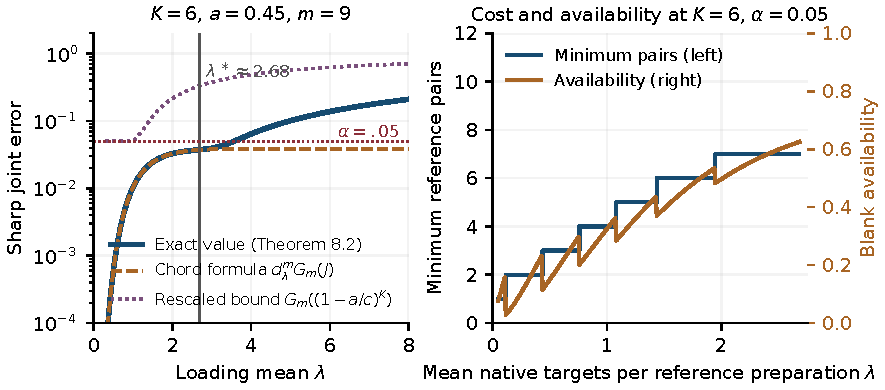
\includegraphics[width=\linewidth]{figures/poisson.pdf}
\caption{Left: the exact value of Theorem~\ref{thm:poissonexact}, evaluated from
the concave envelope, against the chord formula \eqref{eq:poissonsharp} and the
rescaled bound \eqref{eq:rescale}. The two agree to plotting accuracy exactly
while criterion \eqref{eq:chordcrit} holds, and separate immediately past
$\lambda^\ast$; the rescaled bound is safe but far above both. Right: minimum
reference pairs and the resulting blank availability against the loading mean,
at $K=6$, $a=.45$, $\alpha=.05$.}
\label{fig:poisson}
\end{figure}

Heavy loading is not harmless. At $\lambda=100$ with deterministic
$X=Y=.05$, $a=.45$, $K=6$ and $m=9$, the complete-event probability is
$(1-e^{-10})^9(.955)^6\ge.758$, fifteen times the nominal $.049877$: many loaded
targets make poor recovery look like successful calibration. This example lies
outside the regime of Corollary~\ref{cor:poissonconvex} and shows why the
loading mean must appear in the theorem rather than in a footnote.

Finally, $\lambda$ is itself an assumption. A dilution from an uncertain stock,
shared dispensing fluctuation, overdispersion, adsorption or competition can
violate it. If $\lambda$ is a fixed unknown in a justified interval inside the
regime of Corollary~\ref{cor:poissonconvex}, the worst-case bound uses its upper
endpoint, since $d_\lambda$ increases in $\lambda$; availability may be reported
at a lower endpoint for a specified source. A shared random loading effect is a
dependence model, not a substitution.

\section{Observation-law mismatch and control false positives}\label{sec:robust}
\subsection{An event-specific perturbation allowance}
Let each actual reference-pair observation law be within total variation
$\varepsilon_C\in[0,1]$ of its ideal law, and the future target observation law
within $\varepsilon_T\in[0,1]$, with independence across actual experiments as
well as ideal ones. Maximal coupling of each whole pair and of the future
observation gives the product allowance
\begin{equation}\label{eq:TV}
\Prob_{\rm actual}(\text{false certificate})
\le\min\{1,B+1-(1-\varepsilon_C)^m(1-\varepsilon_T)\}
\le\min\{1,B+m\varepsilon_C+\varepsilon_T\},
\end{equation}
where $B$ is any valid ideal bound. This is correct but wasteful, because it
adds the whole coupling defect to a bound that was itself a maximum over
sources. A bound exceeding $\alpha$ means only that \emph{that bound} no longer
certifies $\alpha$; it does not show the actual error exceeds $\alpha$.

\begin{proposition}[Event-specific allowance]\label{prop:robust}
Under the same perturbation class,
\begin{equation}\label{eq:robust}
\Prob_{\rm actual}(\text{false certificate})\le
\mathcal R_m(H;\varepsilon_C,\varepsilon_T):=\max_{0\le w\le1}
\big[\min(1,w+\varepsilon_C)\big]^m\min\{1,1-(1-H)w+\varepsilon_T\},
\end{equation}
and for $H<1$ the maximum is attained in the five-point set consisting of $0$,
$1$, $\varepsilon_T/(1-H)$, $1-\varepsilon_C$ and
$\frac{m(1+\varepsilon_T)}{(m+1)(1-H)}-\frac{\varepsilon_C}{m+1}$, so
\eqref{eq:robust} is an exact finite evaluation for rational inputs.
\end{proposition}
\begin{proof}
Actual pair acceptance is at most $\min(1,w+\varepsilon_C)$ and the actual
all-negative probability at most $\min(1,R_N+\varepsilon_T)\le
\min(1,1-(1-H)w+\varepsilon_T)$ by \eqref{eq:reduction}; the two events are
independent, and maximizing over the ideal source parameter $w$ gives
\eqref{eq:robust}. For the critical set write $c=1-H$ and $A=1+c\varepsilon_C
+\varepsilon_T$. On $\{w\le\varepsilon_T/c\}$ the second factor is capped and the
objective increases in $w$; on $\{w\ge1-\varepsilon_C\}$ the first factor is
capped and the objective decreases; in between the objective is
$u^m(A-cu)$ with $u=w+\varepsilon_C$, which is unimodal with stationary point
$u=mA/((m+1)c)$. The listed points include every endpoint, cap transition and
interior stationary point.
\end{proof}

When both optima lie in the uncapped interior branch, \eqref{eq:robust}
simplifies to
\begin{equation}\label{eq:robustclosed}
\mathcal R_m=G_m(H)\big[1+(1-H)\varepsilon_C+\varepsilon_T\big]^{m+1},
\end{equation}
an inflation by a power $m+1$ of a quantity within $O(\varepsilon)$ of one,
rather than the additive $m\varepsilon_C+\varepsilon_T$ of \eqref{eq:TV}. The
improvement is an order of magnitude at the scales that matter.

\begin{table}[tb]
\centering\small
\caption{Sensitivity of the $K=6$ example to observation-law mismatch, with
$\varepsilon_C=\varepsilon_T=\varepsilon$. The perturbations are illustrative
budgets, not estimated assay errors. ``Meets'' refers to the event-specific
column.}
\label{tab:sensitivity}
\begin{tabular}{@{}rrrrrl@{}}\toprule
Pairs $m$ & $\varepsilon$ & Ideal $G_m(H)$ & Product bound \eqref{eq:TV}
& Event-specific \eqref{eq:robust} & Meets $.05$?\\\midrule
\tableinput sensitivity_rows.tex
\bottomrule\end{tabular}
\end{table}

Table~\ref{tab:sensitivity} shows the practical consequence. At nine pairs and
$\varepsilon=10^{-4}$ the product allowance gives $.050877$ and stops
certifying, while the event-specific bound gives $.049976$ and still certifies;
the apparent fragility at that budget was an artifact of the cruder bound. The
genuine fragility appears at $\varepsilon=10^{-3}$. Ten pairs give a less brittle
design: 20 reference preparations, ideal blank availability
$.96^{10}\approx.664833$, and a bound below $.05$ even at a $3\times10^{-3}$
budget. Note that increasing $m$ reduces ideal error but multiplies the exponent
in \eqref{eq:robustclosed}, so $m$ should be selected against a stated
error-and-availability objective using \eqref{eq:robust}, not by minimizing ideal
error alone.

This remains a conditional sensitivity calculation. No experiment here
establishes that a real assay meets such budgets, and pipetting coefficients of
variation, recovery percentage errors and fluorescence errors are not numerically
interchangeable with total variation distance. If dependence rather than marginal
accuracy is the uncertainty, per-experiment budgets are insufficient and the
joint law must be constrained.

\subsection{Spurious positives: an exact model and a closed form}
Suppose each reference channel additionally reports a spurious positive with
probability $\eta_1,\eta_2$, independent of true recoveries and across
experiments, so that the observed outcomes are $A'=A\lor C_1$ and $B'=B\lor C_2$.
Writing
\begin{equation}\label{eq:kappa}
\kappa=1-(1-\eta_1)(1-\eta_2)
\end{equation}
for the probability that a pair shows at least one spurious positive, the
observed pair acceptance is
\begin{equation}\label{eq:kappaaccept}
\widetilde w=1-(1-\eta_1)(1-\eta_2)(1-w)=\kappa+(1-\kappa)w.
\end{equation}
If the target experiment has independent probability $\eta_T$ of a spurious
positive, its observed all-negative probability is $(1-\eta_T)R_N$. For
conservative control of the exclusion error one should not rely on a beneficial
target artifact whose probability is unknown from below, so we take $\eta_T=0$.

At first sight \eqref{eq:kappaaccept} creates a new optimization problem. It does
not.

\begin{proposition}[Exact reduction and closed form]\label{prop:fp}
Let $0\le\kappa<1$ and $0\le H\le1$, and put
\begin{equation}\label{eq:AHprime}
A_\kappa=\frac{1-\kappa H}{1-\kappa},\qquad
H_\kappa=\frac{H(1-\kappa)}{1-\kappa H}.
\end{equation}
Then for every $w$ and every $m$,
\begin{equation}\label{eq:fpreduce}
[\kappa+(1-\kappa)w]^m\big[1-(1-H)w\big]
=A_\kappa\cdot v^m\big[1-(1-H_\kappa)v\big],\qquad v=\kappa+(1-\kappa)w,
\end{equation}
so the sharp complete-event error under this model is at most
$A_\kappa G_m(H_\kappa)$, with equality whenever the maximizer
$v_*=\min\{1,m(1-\kappa H)/[(m+1)(1-H)]\}$ satisfies $v_*\ge\kappa$; otherwise
it equals $\kappa^m$. In particular $\kappa=0$ recovers Theorem~\ref{thm:main},
and in the interior branch
\begin{equation}\label{eq:fpclosed}
A_\kappa G_m(H_\kappa)=\frac{m^m(1-\kappa H)^{m+1}}
{(m+1)^{m+1}(1-H)^m(1-\kappa)} .
\end{equation}
\end{proposition}
\begin{proof}
Substituting $w=(v-\kappa)/(1-\kappa)$ gives
$1-(1-H)w=[1-\kappa H-(1-H)v]/(1-\kappa)=A_\kappa[1-(1-H_\kappa)v]$, since
$1-H_\kappa=(1-H)/(1-\kappa H)$; this is \eqref{eq:fpreduce}. As $w$ ranges over
$[0,1]$, $v$ ranges over $[\kappa,1]\subseteq[0,1]$, so the maximum is at most
$A_\kappa G_m(H_\kappa)$ by Theorem~\ref{thm:scalar}, with equality when the
unconstrained maximizer is admissible; the stated $v_*$ is
Theorem~\ref{thm:scalar}'s maximizer after simplifying $1-H_\kappa$. When
$v_*<\kappa$ the objective is decreasing on $[\kappa,1]$ and the maximum is at
$v=\kappa$, i.e.\ $w=0$, where the value is $\kappa^m$. For
\eqref{eq:fpclosed}, substitute $(1-H_\kappa)^m=(1-H)^m/(1-\kappa H)^m$ into the
interior branch of \eqref{eq:G} and multiply by
$A_\kappa=(1-\kappa H)/(1-\kappa)$.
\end{proof}

At total recovery failure $w=0$ the gate still passes with probability
$\kappa^m$, which is why positive reference signals without specificity controls
are insufficient evidence. Quantitatively, Table~\ref{tab:specificity} evaluates
\eqref{eq:fpclosed} at the worked design.

\begin{table}[tb]
\centering\small
\caption{Effect of spurious control positives on the $K=6$, $m=9$, $a=.45$
example. $\kappa$ is the probability that a reference pair shows at least one
spurious positive; $\eta_T=0$ is assumed for the target.}
\label{tab:specificity}
\begin{tabular}{@{}rrrl@{}}\toprule
Pair false-positive rate $\kappa$ & decimal & Sharp joint error & Meets $.05$?\\\midrule
\tableinput specificity_rows.tex
\bottomrule\end{tabular}
\end{table}

The specificity budget is severe: the nine-pair design tolerates
$\kappa\le1/300$ and fails at $\kappa=1/250$. Compared with the transport budget
of Table~\ref{tab:sensitivity}, which tolerates $\varepsilon=10^{-4}$
comfortably, control false positives are the binding practical constraint on
this design, and they should be budgeted first.

\subsection{What negative controls establish}
Extraction blanks, no-template controls and matrix-matched negatives interrogate
different routes to false positivity. They do not measure native recovery by
themselves, they must be counted in the resource budget, and they cannot be added
silently as free validation.

If $n$ independent negative-control \emph{pairs} show no spurious pair pass, the
exact one-sided binomial upper confidence bound at failure probability $\delta$
is the Clopper--Pearson value \cite{clopper1934}
\begin{equation}\label{eq:cp}
\kappa_U=1-\delta^{1/n}.
\end{equation}
At $n=96$ and $\delta=.05$ this is $\kappa_U\approx.030724$, which by
Table~\ref{tab:specificity} is roughly a factor of nine too large to support the
nine-pair design. Certifying $\kappa\le1/300$ at $\delta=.05$ requires
$(1-1/300)^n\le1/20$, that is $n=898$ clean independent control pairs. Zero
observed positives do not establish a zero false-positive rate, and pairing,
matrix matching and independent sampling remain assumptions. If a data-dependent
bound for $\kappa$ is used to choose a reporting policy, its coverage failure
belongs in the procedure's error budget; plugging an estimated rate into
\eqref{eq:fpclosed} is not justified.

This is a prospective validation requirement, not a validated dataset. It is also
the clearest instance of a general point: the cheap part of this design is the
mathematics, and the expensive part is the evidence that its premises hold.

\section{What stronger source information buys}\label{sec:constrained}
The corner laws of Theorem~\ref{thm:main} show what an unrestricted model
permits. They do not assert that extreme failure is common. Excluding them
requires evidence expressed as a mathematical restriction, and different
restrictions buy very different amounts.

\subsection{Nonnegative covariance alone buys nothing}
Two distinctions matter. First, $q>0$ is not positive correlation: nonnegative
covariance means $q\ge p_1p_2$. Second, nonnegative covariance \emph{alone},
with unrestricted marginal means, does not improve
Theorem~\ref{thm:main} at all. Take $Y\equiv0$ and $X$ Bernoulli with mean $z_*$:
then $q=0=p_1p_2$, the covariance is zero, and the source attains $G_m(H)$
exactly. An assumption that protocols are comparable, or that recoveries are
similar, therefore has no content unless it constrains the marginals.

\subsection{Equal means and nonnegative covariance}
\begin{theorem}[Sharp value under a constrained source class]\label{thm:constrained}
Restrict the source class to equal marginal means $p_1=p_2=p$ and nonnegative
covariance $q\ge p^2$. Then for balanced $a\le1/2$, with $H,J$ as in
\eqref{eq:HJ},
\begin{equation}\label{eq:constrained}
\sup\Prob(\mathcal A_m\cap\Neg)
=\max_{0\le p\le1}(2p-p^2)^m\big[(1-p)^2+2p(1-p)H+p^2J\big],
\end{equation}
attained by independent Bernoulli recovery coordinates with success probability
$p$, at $N=K$.
\end{theorem}
\begin{proof}
By \eqref{eq:reduction} the envelope is $1-w(1-H)-q(H-J)$ with $w=2p-q$, which is
nonincreasing in $q$ at fixed $w$ because $H\ge J$. At fixed $w$ the constraint
$q=2p-w\ge p^2$ forces $p\ge1-\sqrt{1-w}$, and $q=2p-w$ increases with $p$, so
$q$ is minimized at $p=1-\sqrt{1-w}$, where $q=p^2$ exactly. The remaining
feasibility constraints \eqref{eq:feasible} hold there, since $p^2\le p$ and
$p^2\ge2p-1$. Hence the extremal source in this class is the independent
Bernoulli law with corner masses $((1-p)^2,p(1-p),p(1-p),p^2)$, for which
$w=2p-p^2$ and the envelope equals $(1-p)^2+2p(1-p)H+p^2J$ by direct expansion.
As $p$ ranges over $[0,1]$, $w=2p-p^2$ ranges over all of $[0,1]$, so no value of
$w$ is lost.
\end{proof}

\subsection{The floor moves from \texorpdfstring{$H$}{H} to
\texorpdfstring{$J$}{J}}
The practical content of Theorem~\ref{thm:constrained} is not the formula but
where its floor sits.

\begin{corollary}[Feasibility threshold]\label{cor:constrainedfloor}
Denote by $G^{\mathrm{cov}}_m$ the right side of \eqref{eq:constrained}. Then
$G^{\mathrm{cov}}_m\ge J$ for every $m$, and $G^{\mathrm{cov}}_m\downarrow J$ as
$m\to\infty$. Consequently, within this source class a level $\alpha$ is
reachable by some finite $m$ if and only if $\alpha>J=(1-2a)^K$, whereas in the
unrestricted class of Theorem~\ref{thm:main} it is reachable if and only if
$\alpha\ge H=(1-a)^K$.
\end{corollary}
\begin{proof}
The value at $p=1$ is exactly $J$, giving the lower bound. For the limit, fix
$\eta\in(0,1)$ and split at $p=1-\eta$: for $p\le1-\eta$ the gate factor
$(2p-p^2)^m=(1-(1-p)^2)^m\le(1-\eta^2)^m\to0$, while for $p\ge1-\eta$ the bracket
is at most $\eta^2+2\eta H+J$. Hence
$\limsup_mG^{\mathrm{cov}}_m\le\eta^2+2\eta H+J$ for every $\eta>0$, so the limit
is $J$. The unrestricted statement is Theorem~\ref{thm:scalar}: $G_m(H)$ is
nonincreasing in $m$ with minimum value $H$, attained once $m\ge1/H-1$.
\end{proof}

This converts an impossibility into a cost. At $a=.45$ and $K=2$ we have
$H=.3025$ and $J=.01$: no reference budget can certify $\alpha=.05$ over
unrestricted recovery laws, but 38 pairs suffice once equal means and
nonnegative covariance are assumed, with sharp value $.04989975$.
Table~\ref{tab:constrained} gives the corresponding counts for
$K=2,\dots,6$, and Figure~\ref{fig:constrained} shows the two floors.

\begin{table}[tb]
\centering\small
\caption{Reference pairs needed for $\alpha=.05$ at $a=.45$, comparing the
unrestricted source class with equal means and nonnegative covariance. The
constrained minima are certified in exact rational arithmetic from both sides.}
\label{tab:constrained}
\begin{tabular}{@{}rrrrrr@{}}\toprule
Null $N\ge K$ & $H=(1-a)^K$ & $J=(1-2a)^K$ & Pairs, unrestricted
& Pairs, constrained & Sharp value\\\midrule
\tableinput constrained_rows.tex
\bottomrule\end{tabular}
\end{table}

\begin{figure}[!htb]
\centering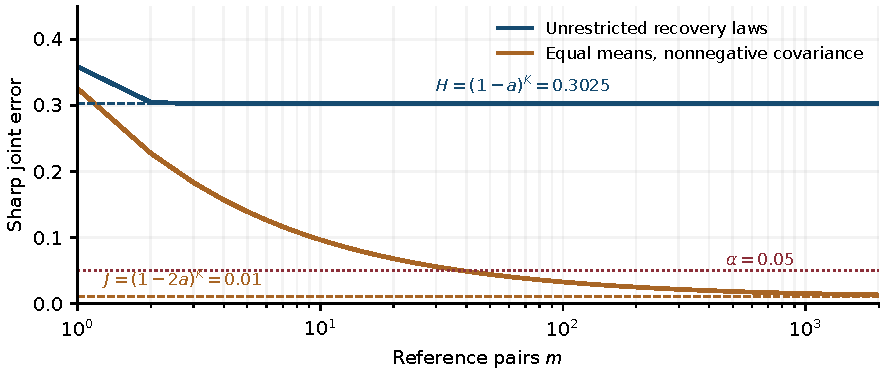
\includegraphics[width=\linewidth]{figures/constrained.pdf}
\caption{Sharp joint error against reference budget at $K=2$, $a=.45$. Over
unrestricted recovery laws the value is pinned at $H=.3025$ for every
$m\ge3$; under equal means and nonnegative covariance it decreases to the floor
$J=.01$ and crosses $\alpha=.05$ at $m=38$.}
\label{fig:constrained}
\end{figure}

The interpretation is concrete. The floor $H$ is the miss probability of a source
in which exactly one preparation works; the floor $J$ is that of a source in
which both do. Assuming equal means and nonnegative covariance is precisely the
assumption that a state in which one preparation systematically works while the
other systematically fails is not the whole story, and the exclusion threshold
that becomes reachable is governed by the total coverage $2a$ rather than the
per-preparation coverage $a$. Whether this transports from a validation
population to actual specimens is an empirical question, and
Corollary~\ref{cor:constrainedfloor} makes explicit exactly how much it is worth
paying to answer it.

Corollary~\ref{cor:poissonconvex} cautions against the opposite error. Its sharp
witness has $X=Y$, so shared all-or-nothing failure can be the limiting
mechanism even under perfect positive dependence. Worst-case behavior is a
property of the observation law, not a fixed picture of antagonistic recoveries.

\section{Relation to detection-capability validation}\label{sec:standards}
Detection-capability validation addresses neighboring but distinct questions. A
blank decision threshold concerns how often blank material produces an apparent
positive, and a limit of detection concerns a low level detected with specified
probability under a defined measurement procedure; CLSI EP17-A2 is the standing
guidance \cite{clsi2012}. The present claim instead bounds false exclusion of a
\emph{count in an original specimen}, over a source model and an explicit
reference-and-target reporting event. These are complementary. A properly
designed whole-process detection study can and should include extraction and
matrix failures, and nothing here shows that such a study is inadequate.

The failure mode we do identify is a modeling one. Suppose a process fails
completely with probability $\rho$ and otherwise detects each of $N$ targets
independently with probability $d$. Its miss probability is
\begin{equation}\label{eq:shared}
\rho+(1-\rho)(1-d)^N,
\end{equation}
whereas an analysis that replaces this by $[1-(1-\rho)d]^N$ resamples the shared
failure for each target and can understate risk by orders of magnitude at
moderate $N$. Equation \eqref{eq:source} is the general form of
\eqref{eq:shared}, and the entire paper is an accounting of the difference.
This diagnoses a mismatch between a model and a process; it does not establish a
defect in a particular standards-compliant study.

The reporting records needed to evaluate the present contract --- sample
processing amounts, extraction replicates and blanks, blank and detection limit
assessment, inhibitors, positive and negative controls, technical replication,
partition volume and copies per partition --- are exactly those enumerated by
MIQE~2.0 \cite{miqe2025} and the digital PCR checklist \cite{dmiqe}. Our bound
complements detection-capability validation by making the original-specimen
denominator, the shared recovery and the reference-based reporting event
explicit. It does not replace blank or detection limit estimation, and it does
not establish that the native-reference transport assumptions hold in any
particular assay.

\section{Interpretation and prospective validation}\label{sec:discussion}
For a fixed recovery law and independent future specimen, whenever the gate has
positive probability,
\[
\Prob(\Neg\mid\mathcal A_m)=R_N.
\]
The small joint error in \eqref{eq:main} is not a claim that the conditional miss
probability after acceptance is equally small, nor a posterior probability that
the specimen contains fewer than $K$ targets. Reference gating controls how often
an experiment issues an erroneous certificate across complete repetitions.

The deployment unit is one reference campaign and one future specimen.
Section~\ref{sec:batch} makes the cost of departing from that unit exact rather
than rhetorical, and the same discipline applies to the other three relaxations:
each of Sections~\ref{sec:poisson}, \ref{sec:robust} and \ref{sec:constrained}
replaces an informal worry with a number that a design can be checked against.
Collecting them, the worked $K=6$ design survives mean-one Poisson loading and
transport budgets of order $10^{-4}$, fails for any batch of two, and requires a
control false-positive rate below $1/300$ that itself needs some 900 clean
control pairs to certify. That profile, not the headline $.0499$, is the honest
summary of what the design can do.

A validation study should use counted native-like inputs and representative
matrices, retain the full four-outcome reference table and invalid records, and
record original volume, usable volume, target-count uncertainty, extraction and
well identities, coverage, and independently sampled batch identifiers. It should
first challenge transport across target forms and volumes, representative
material loss, competition, reference classification, and dependence across
nominally independent pairs. The relevant gate quantity is $w=\Prob(A\lor B)$,
while $q$ remains useful for allocation. A convenient downstream spike is not
sufficient evidence, and reporting compliance does not prove native transport. No
linked native-reference dataset is supplied here; existing readout-processing
records without original-volume and extraction linkage cannot establish the
required law.

The practical limitation is structural. At the endpoint, an adverse source passes
every reference pair and still misses finite targets because material allocation
and preparation recovery remain imperfect; more calibration cannot remove that
floor, and Corollary~\ref{cor:floor} shows the same phenomenon governs batch
reuse. In the interior regime, partial acceptance balances a poorer future assay.
The exact formulas identify whether additional independent references, improved
unique coverage, stronger recovery information or a changed exclusion threshold
can meet an intended budget. They do not warrant a universal preference for
splitting, and they do not license a claim about disease absence.

Several questions remain open. The concave-envelope problem of
Theorem~\ref{thm:poissonexact} is solved in closed form only when the envelope
degenerates to a chord; a classification of the tangency point $\tau$ outside
that regime would complete it.
Multiple-testing procedures designed for this architecture, rather than inherited
from it, could plausibly beat Corollary~\ref{cor:floor} by conditioning on the
calibration record. Adaptive policies that choose the next experiment after a
history of negatives need a sequential analysis that we have deliberately not
attempted.

\appendix
\section{Formal scope and reproducibility}\label{app:formal}
The ordinary proofs above are self-contained. The accompanying Lean~4
development \cite{lean4,mathlib2020} uses the repository's pinned Lean~4.30.0 and
mathlib environment, with warnings treated as errors. Its finite-mixture model
admits any finite number of continuous-valued recovery states. Only the standard
axioms \lean{propext}, \lean{Classical.choice} and \lean{Quot.sound} occur; no
\lean{sorry}, additional axiom, native decision procedure or numerical oracle is
used.

\begin{table}[htb]
\centering\small
\caption{Claim-to-declaration map. All declarations live in the Lean namespace
\texttt{SpecimenReliability}; the thirteen modules form one dependency chain
rooted at \texttt{Source.lean}. The last three modules are additions of the
present paper.}
\label{tab:formalmap}
\newcolumntype{L}[1]{>{\raggedright\arraybackslash}p{#1}}
\begin{tabular}{@{}L{0.40\linewidth}L{0.55\linewidth}@{}}\toprule
Paper claim & Lean declarations\\\midrule
Conserved target paths and the source law \eqref{eq:source}; monotonicity in the
count &
\lean{path_normalized}, \lean{path_nonneg}, \lean{negative_histories},
\lean{source_law}, \lean{risk_count_mono}\\[2pt]
Sharp moment envelope, Theorem~\ref{thm:envelope} &
\lean{pointwise_envelope}, \lean{sharp_upper}, \lean{envelope_attained},
\lean{corners_moments}, \lean{corners_nonneg}\\[2pt]
Paired reference law \eqref{eq:reference} and feasible moments \eqref{eq:feasible} &
\lean{reference_law}, \lean{reference_as_corners}, \lean{moments_feasible}\\[2pt]
Complete-event identity \eqref{eq:joint} &
\lean{accepted_identity}\\[2pt]
Scalar maximum, Theorem~\ref{thm:scalar} &
\lean{gate_opt_properties}, \lean{gate_maximum}, \lean{gate_endpoint},
\lean{gate_interior_formula}\\[2pt]
Sharp calibrated count exclusion, Theorem~\ref{thm:main} &
\lean{accepted_reduction}, \lean{accepted_general}, \lean{general_attainment},
\lean{witness_family_valid}\\[2pt]
Three-pair corollary, Corollary~\ref{cor:cubic} &
\lean{cubic_gate_bound}, \lean{accepted_resolution}, \lean{accepted_sharp}\\[2pt]
Reporting availability, Section~\ref{sec:gate} &
\lean{accepted_blank_rate}, \lean{utility_comparison}, \lean{utility_examples},
\lean{discordance_subset}\\[2pt]
Single-preparation comparator \eqref{eq:single} &
\lean{single_identity}, \lean{single_general}, \lean{single_attainment},
\lean{single_witness_valid}\\[2pt]
Exact worked thresholds, Table~\ref{tab:thresholds} &
\lean{worked_bounds}\\[2pt]
Batch composition identity behind Theorem~\ref{thm:batch} &
\lean{atLeastOne_law}, \lean{batch_identity}\\[2pt]
Floor attainment, Corollary~\ref{cor:floor} &
\lean{batch_witness}, \lean{batch_witness_valid}\\[2pt]
Two-specimen impossibility at $K=6$, $a=.45$, Section~\ref{sec:batch} &
\lean{batch_floor_exceeds}\\[2pt]
False-positive reduction and bound, Proposition~\ref{prop:fp} &
\lean{fp_reduction}, \lean{fp_bound}\\[2pt]
Specificity thresholds, Table~\ref{tab:specificity} &
\lean{fp_example_safe}, \lean{fp_example_unsafe}\\[2pt]
Poisson comparison and the guarantee for $\lambda\le1$,
Proposition~\ref{prop:poissonsafe} &
\lean{poisson_pointwise}, \lean{poisson_accept_le},
\lean{poisson_accept_nonneg}, \lean{poisson_general}\\
\bottomrule\end{tabular}
\end{table}


The following are \emph{not} mechanized and are established by the ordinary
proofs given above: the unequal-allocation results of Section~\ref{sec:choice};
the extension from finite mixtures to arbitrary probability laws on the unit
square by integrating the same pointwise inequalities; the asymptotic
expansions of Section~\ref{sec:examples}; the closed form
\eqref{eq:batchform} and the limit in Corollary~\ref{cor:floor} (the batch
identity, the attaining witness and the numerical impossibility \emph{are}
mechanized); the coupling arguments of Section~\ref{sec:robust} including
Proposition~\ref{prop:robust}; the concave-envelope reduction
Theorem~\ref{thm:poissonexact} and its Corollary~\ref{cor:poissonconvex} (the
conservative transport Proposition~\ref{prop:poissonsafe} \emph{is} mechanized);
the sharpness half of Proposition~\ref{prop:fp} (its reduction and upper bound
\emph{are} mechanized); and Theorem~\ref{thm:constrained} with
Corollary~\ref{cor:constrainedfloor}. Numerical plots illustrate established
formulas; finite numerical checks do not prove continuum claims, and no assertion
of biological validity follows from formal verification.

Every number printed in this manuscript is regenerated and re-checked by
\texttt{check\_paper.py}. The script finally re-reads \texttt{main.tex} itself
and verifies that each decimal literal in the prose is the correctly rounded form
of a quantity it computed, so no figure quoted in the text is unaccounted for. It
uses exact rational arithmetic wherever the
quantity is rational and certified rational Taylor enclosures for the
exponentials in Section~\ref{sec:poisson}, so each integer threshold reported is
a proved decision. The minimum pair counts of Table~\ref{tab:constrained} are
certified from both sides: an adaptive exact-rational bisection proves the
constrained maximum lies below $\alpha$ at the stated $m$, and an exact rational
witness proves it does not at $m-1$. The one quantity that is irrational by
nature, the interior branch of \eqref{eq:batchform}, is evaluated in double
precision and labelled as such in Table~\ref{tab:batch}; the reachability
decisions in that section depend only on the exact floor.
\texttt{make\_figures.py} rebuilds all five figures. Build instructions,
verification commands and the claim-to-declaration map are in the accompanying
\texttt{BUILD.md}.

\bibliographystyle{plainnat}
\bibliography{references}
\end{document}
